\documentclass[notitlepage]{article}
\usepackage{graphicx}
\usepackage{bmpsize}
\usepackage{color}
\usepackage{courier}
\usepackage{listings}
\usepackage{times}
\usepackage[T1]{fontenc}
\usepackage{textcomp}
\usepackage{fullpage}
\usepackage{hhline}
\usepackage{tabular x}
\usepackage{mdframed}
\usepackage{enumerate}
\usepackage{titlesec}
\usepackage{hyperref}
\usepackage[clock]{ifsym}

\lstset{language=VHDL}
\lstset{basicstyle=\normalsize\ttfamily,breaklines=true}
\graphicspath{ {img/} }
\newcommand{\sectionbreak}{\clearpage}
\newcommand{\infosign}{\fontencoding{U}\fontfamily{futs}\huge\selectfont\char 116\relax}
\newcommand{\warningsign}{\fontencoding{U}\fontfamily{futs}\Large\selectfont\char 66\relax}
\newcommand{\dangersign}{\fontencoding{U}\fontfamily{futs}\huge\selectfont\char 76\relax}
\newmdenv[linecolor=black,skipabove=\topsep,skipbelow=\topsep,
leftmargin=0pt,rightmargin=0pt,
innerleftmargin=5pt,innerrightmargin=5pt]{infobox}
\makeatletter
\newcommand*{\toccontents}{\@starttoc{toc}}
\makeatother

\begin{document}

\title{\huge{\texttt{ratload}\\ Installation and Use}}
\author{
  Jacob Hladky\\
  California Polytechnic State University\\
  San Luis Obispo, CA\\
  \texttt{jhladky@calpoly.edu}
}
\date{\today}
\maketitle

\toccontents

\pagenumbering{arabic}

\section{Introduction}
\texttt{Ratload} is a system for loading new RAT assembly programs on to the RAT CPU without the need for resynthesis.\\\\
The system consists of two components: a computer program and a set of VHDL modules. This guide will detail how to install and use --- and optionally troubleshoot --- both. It is necesssary to follow the instructions in both \emph{Integration} sections, and then either of the \emph{Installation} sections, depending on the target platform. \texttt{Ratload} is compatible with Windows and Linux.

\subsection{Requirements}
If you have a Nexys 2 board --- You will need a serial cable. If your computer does not have a serial port, then you will need a USB-to-serial adapter. Here's an example: \url{http://amzn.com/B0007T27H8}. Any adapter will do as long as you have the right drivers for it.\\
If you have a Nexys 3 board --- No serial cable is required, as an onboard FTDI chip provides serial emulation.\\\\
Do not integrate ratload into your RAT CPU until all the major components of the CPU are in place, and you have a good understanding of how they fit together. Understanding how the RAT architecture handles I/O and interrupts will make integration much easier.

\subsection{Project Manifest}
The following is a listing of each file in the \texttt{ratload} system and a brief description of the file's contents and purpose.
\begin{itemize}
\item \texttt{README.pdf} This guide.
\item \texttt{vhdl/uart.vhd} Top-Level UART VHDL module. Required for communication with host computer.
\item \texttt{vhdl/RS232RefComp.vhd} UART VHDL module. Required for communication with host computer.
\item \texttt{vhdl/ascii\_to\_int.vhd} VHDL module to convert ASCII-encoded hexidecimal numbers into binary.
\item \texttt{vhdl/prog\_rom.vhd} Replacement prog\_rom module for the RAT CPU.
\item \texttt{vhdl/interceptor.vhd} VHDL module related to the internal operation of the prog\_rom.
\item \texttt{vhdl/prog\_ram.vhd} VHDL module related to the internal operation of the prog\_rom.
\item \texttt{vhdl/real\_prog\_rom.vhd} VHDL module related to the internal operation of the prog\_rom.
\item \texttt{vhdl/serial\_test.vhd} A special prog\_rom module used to test the functionality of the UART.
\item \texttt{bin/ratload\_Windows/} Windows graphical version of the ratload program. The files in this directory are all in support of the Windows ratload program and will not be described individually.
\item \texttt{bin/ratload\_Windows\_x86.exe} Windows command-line version of the ratload program.
\item \texttt{bin/ratload\_Linux\_x86\_64} Linux command-line version of the ratload program.
\end{itemize}
There is no graphical ratload program for Linux.

\begin{infobox}
  {\infosign} Running \texttt{ratload} on OS X is possible, but unsupported. You will have to build the program yourself. For more information see Section~\ref{sec:source_build}.
\end{infobox}

\subsection{Bug Reporting}
All programs have bugs. \texttt{ratload} is beta software and is no exception. If you encounter a bug in the ratload program, please contact the author. It is also possible (albeit significantly less likely) that you find a bug in the project VHDL modules. If you do please verify the bug via simulation and report it immediately so it can be fixed.\\\\
Since you are writing the mechanics of the CPU itself, it is possible for very odd bugs to happen, and for those bugs to interact with \texttt{ratload} in bizarre ways\ldots However \texttt{ratload} has been thoroughly tested and is free of any major bugs.

\subsection{Contact}
If you have any questions about the project itself, or suggestions for improvement for this guide, please contact the author at jhladky@calpoly.edu. This project licensed under the MIT license and the complete source code --- including the \LaTeX ~source for this guide --- is available at \url{http://www.github.com/jhladky/ratload}.

\section{Adding the New RAT Wrapper}
\texttt{Ratload} requires a UART to communicate with the host computer, which is provided as part of a new RAT wrapper module, which will replace your current wrapper. The new RAT wrapper provides access to the LEDs, and the buttons, and the switches. If you want to add any more I/O devices, such as the 7-segment display of the VGA driver buffer, then you will need to add them manually.

\begin{infobox}
  {\infosign} UART stands for ``Universal Asynchronous Receiver-Transmitter'', which you may recognize as another name for a serial port. The UART can be used outside of the \texttt{ratload} project as well. Consider using the UART in your own final project!
\end{infobox}

\subsection{Integration with RAT CPU}

\begin {enumerate}
\item In the Xilinx ISE Environment, go to \textbf{Project \textgreater Add Copy of Source}. Navigate to the \texttt{ratload} project directory (where this README is located), and then to the ``vhd'' folder. Select the following modules:
\begin{itemize}
\item \texttt{rat\_wrapper.vhd}
\item \texttt{uart.vhd}
\item \texttt{ascii\_to\_int.vhd}
\item \texttt{int\_to\_ascii.vhd}
\item \texttt{RS232RefComp.vhd}
\end{itemize}

\begin{infobox}
  {\warningsign} This is a destructive action and will overwrite any files already in your project directory that have a name identical to the files being added. You will have to confirm that you want to add the files.
\end{infobox}

Click \textbf{Open}. Another dialog box will pop up confirming you want to add these files. Click \textbf{OK}.

\item In the rat\_wrapper.ucf file (your title may differ slightly), add the following NETs if you have a Nexys 2 board:
\begin{lstlisting}
NET "TXD" LOC = P9;
NET "RXD" LOC = U6;
\end{lstlisting}

If you have a Nexys 3 board, then add these lines instead:
\begin{lstlisting}
NET "TXD" LOC = XX;
NET "RXD" LOC = XX;
\end{lstlisting}

\item That is all that's necessary to add the new RAT wrapper. However the signal names of your \textbf{RAT CPU module} may differ from those declared in the RAT wrapper. Change the signal names in the RAT wrapper as necessary and make sure you can generate a bit file.
\end{enumerate}

\subsection{Verification}
This section covers a quick test of the UART module you just integrated into your RAT CPU. If the test in this section is not 100\% successful \textbf{DO NOT CONTINUE}. Go back and double check that you have integrated the UART properly. If the UART continues not to work, see Section~\ref{sec:troubleshooting}. \texttt{Ratload} \textbf{WILL NOT WORK} unless your UART bahaves exactly as expected!

\begin{enumerate}
\item Replace your current prog\_rom module with the prog\_rom module in the ``serial\_test.vhd'' file, in the ``vhdl'' folder. Then program your Nexys board with the new bit file.
\item Hook up the serial cable to the Nexys and the host computer. If the test indicates ``PASS'', then you can skip Section~\ref{sec:troubleshooting}. If it says anything else, go back and make sure you followed the integration instructions properly.

\begin{infobox}
  {\infosign} This step involves running the ratload program. For more information about installing and running the ratload program see Sections 4 and 5. % FIX THE REF HERE...
\end{infobox}

  \begin{enumerate}[a.]
  \item \textbf{Graphical version (Windows only) ---} Select the proper serial device from the dropdown menu. Then go to \textbf{File \textgreater Run Serial Test}. The program will then attempt to communicate with the Nexys board via the serial cable.

  \item \textbf{Command-line version ---} Run ratload in test mode like so: \texttt{ratload -d /dev/<serial device> -{}-test}
  \end{enumerate}
\end{enumerate}

\subsection{Troubleshooting}
\label{sec:troubleshooting}
The easiest way to troubleshoot the UART module is to break out an actual serial console and see what it's sending to the computer. So that's what we're going to do. You will need to know what your serial device is called on your computer. To do so see Section~\ref{sec:serial_id}.
\subsubsection{Obtaining a serial console}
\begin{itemize}
\item \textbf{Windows users --- } A good serial console for windows is putty. Download it here: \url{http://bit.ly/1jsQjnt}
\item \textbf{Linux users --- } Install minicom with your package manager. If you are using a debian-based disto that looks like: \texttt{sudo apt-get install minicom}.
\end{itemize}

\begin{figure}[ht!]
  \centering
  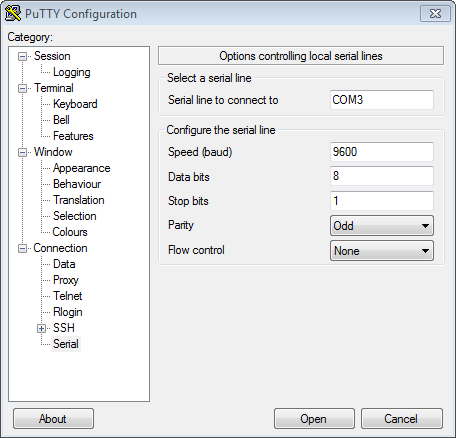
\includegraphics[width=0.5\textwidth]{fig0.png}
  \caption{The correct settings to use with Putty}
  \label{fig:putty}
\end{figure}

\subsubsection{Configuring the proper serial console settings}
\begin{itemize}
\item \textbf{Windows users --- }
  Run putty. From the \textbf{Connection Type} options, select the \textbf{Serial} radio button. Enter the COM port of your serial device in the \textbf{Serial Line} box. Before you can connect on the serial line you need to make sure it has the correct settings. Make your putty settings look like they do in Figure~\ref{fig:putty}. Remember that your COM port may differ. After you have entered the correct settings click \textbf{Open}.

\item \textbf{Linux users --- } Start minicom from the terminal in config mode by using the \texttt{-s} flag, like so: \texttt{minicom -s}. Use your keyboard to navigate the configuration menu that pops up. Select the \textbf{Serial Port Setup} option. Make your minicom settings look like they do in Figure~\ref{fig:minicom}. Remember that your serial device and ``Lockfile Location'' may differ (you can ignore ``Lockfile Location'', actually). After you gave entered the correct settings hit escape until minicom dumps you out to the serial console window.

\begin{figure}[ht!]
  \centering
  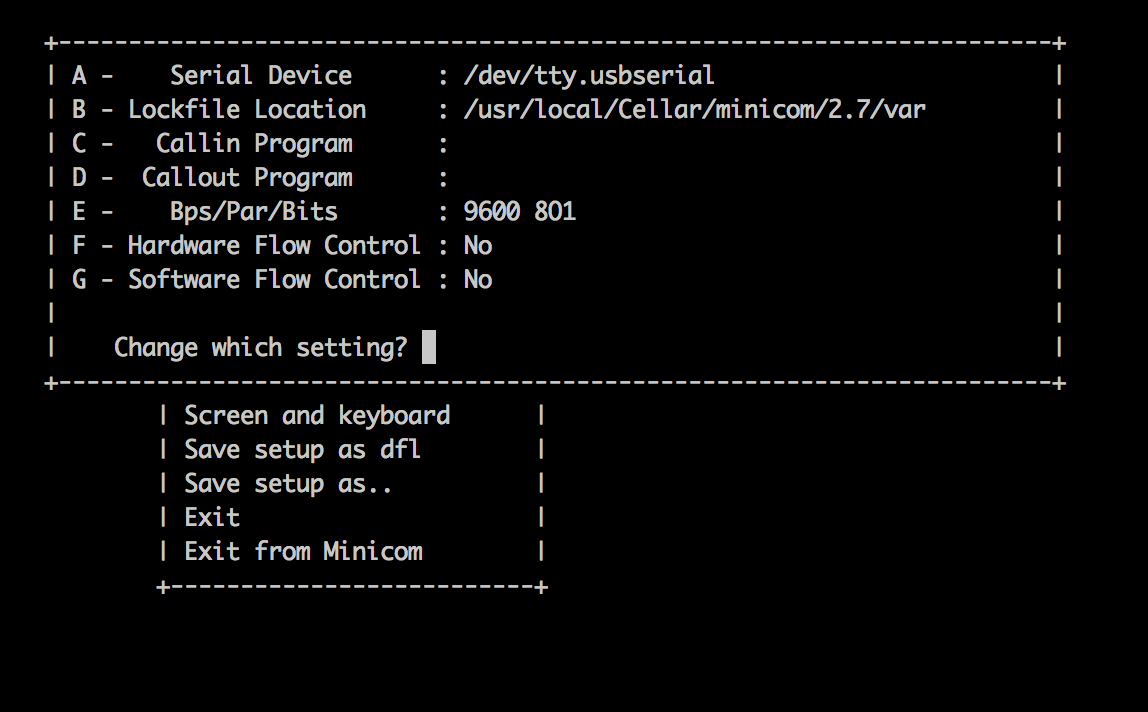
\includegraphics[width=0.5\textwidth]{fig1.png}
  \caption{The correct settings to use with minicom}
  \label{fig:minicom}
\end{figure}
\end{itemize}

\subsubsection{Using the serial console to troubleshoot the UART}
Once you have your serial console up and running flash your Nexys board with your bit file that has the serial test program on it. (Make sure you've connected the Nexys board to your computer with the serial cable).\\\\
Send some data to the UART from the serial console. This is done by typing in the serial console. The behavior of the serial test program is as follows:
\begin{enumerate}
\item Get an ASCII-encoded byte from the UART
\item Convert that byte to binary
\item Send that byte back to the computer.
\end{enumerate}
So for example if you type in an ASCII '1' in the serial console, the serial test program will return the number 1. The number '1' in ASCII is in a class of characters called ``control characters'', so the serial console should display some symbol indicating it received a control character.\\\\
So you are looking for the following behavior when interacting with the serial test program:
\begin{enumerate}
\item Send 1 ASCII-encoded byte
\item Receive \textbf{exactly 1} byte back, that is the ASCII-character ``decoded''.
\end{enumerate}
If you receive two characters back, if you receive no characters back, if you receive a flood of characters back, or anything that is not that exact sequence, then you have integrated the UART incorrectly.

\section{Adding the New Prog\_Rom module}
Once you have added the UART and verified that it is functioning correctly, the remaining steps are simple.
\begin{enumerate}
\item Go to \textbf{Project \textgreater Add Copy of Source}. Navigate to the \texttt{ratload} directory again and then to the same ``vhdl'' folder. Select the ``prog\_rom.vhd'', ``prog\_ram.vhd'', ``real\_prog\_rom.vhd'', and ``interceptor.vhd'' files and click \textbf{Open}. Another dialog box will pop up confirming you want to add these files. Click \textbf{OK}.

\begin{infobox}
  {\warningsign} This is a destructive action and will overwrite any files already in your project directory that have a name identical to the files being added e.g. any existing prog\_rom.vhd file will be overwritten by the \texttt{ratload} prog\_rom.vhd file.
\end{infobox}

\item In the architecture section of the rat\_cpu module, edit the componet declaration for the prog\_rom module. Add the following line:\\
  \centerline{\texttt{TRISTATE\_IN : in STD\_LOGIC\_VECTOR(7 downto 0)}}

\item In the same file, edit the port map decaration for the prog\_rom module. Map the signal for the RAT CPU's tristate bus into to the prog\_rom module's tristate bus. The RAT CPU's ``tristate\_bus'' may be called the ``MULTI\_BUS'' in your CPU. (Regardless of its name, this is the bux that connects the ALU, the program counter, the scratch pad, and others.) That line will look similar to this:\\
  \centerline{\texttt{tristate\_in =\textgreater ~tristate\_bus\_sig(7 downto 0),}}

\item Synthesize and generate a bit file for your newly integrated system. That's it! \texttt{Ratload} should work on your CPU now. The next sections cover installing and using the ratload program.
\end{enumerate}

\section{Installing the Ratload Program}
Installation is really easy. For all platforms the command-line ratload binary is self-contained. Installation consists of copying the program to a location convenient to you. Make sure to choose the binary corresponding to your platform. Linux users need ``ratload\_Linux\_x86\_64'', and Windows users need ``ratload\_Windows\_x86.exe''. The Windows binary is inside the ``ratload\_Windows'' directory. Instructions for using the grapical version of ratload (Windows only) and for building from source and included below.

\subsection{Graphical ratload (Windows only)}
The graphical version of the ratload program is located in the folder ``ratload\_Windows''. Copy the entire folder somewhere useful to you. The graphical program will not work without the container folder. There is no other installation step.

\subsection{Building from source}
\label{sec:source_build}
\begin{infobox}
  {\infosign} This section is very technical and is advanced users only. If you do not have a solid understanding of the software build process it is safe to ignore this section.
\end{infobox}

Ratload is written in Java and is compiled to assembly by the GNU Compiler for Java (GCJ). Libgcj and Libgcc are statically linked into the binary on Windows and Linux (which is why the binary is so large). It is possible to build and link ratload dynamically on Linux and OS X. In fact, ratload should build on any POSIX-compliant OS. The source is available at \url{http://github.com/jhladky/ratload}, in the \texttt{src} folder.

\section{Use}
Up until now, you've probably followed this pattern when developing your assembly language programs:
\begin{enumerate}
\item Run your assembly repeatedly in the ratsim program until it produces a prog\_rom.vhd file and seems to be bug free.
\item Add the new prog\_rom.vhd file to your project, replacing the old one.
\item Resynthesize the entire project and reprogram the bit file onto your Nexys board.
\item Repeat ad infinitum.
\end{enumerate}
The steps you have just followed to integrate the vhd files into your RAT CPU, and to install the ratload program onto your computer, will dramatically change this pattern. From now on you do not need to resynthesize your project when ratsim generates a new prog\_rom.vhd file, nor is it necessary to copy that new file into your project. In fact, \textbf{making any more changes to the prog\_rom.vhd file in your project directory will break \texttt{ratload}}.\\\\
This section contains instructions for identifying the serial device you need to use to communicate with the Nexys board, an overview of the \texttt{ratload} procedure, and instructions on using either the command-line or the graphical (Windows only) ratload program.

\subsection{Identifying your Serial Device}
\label{sec:serial_id}
How you identify your serial device will depend on what Nexys board you have as well as whether you are using a USB-serial adapter or not. Before you identify your serial device you need to make sure you have the correct drivers installed for it. This sounds a lot more complicated than it really is. Follow either of the following sections based on which Nexys board version you have to make sure you have the right drivers installed.

\subsubsection{Nexys 2}
If you have a serial port on your computer, congratulations, you are using a computer from the 20th century! Your OS almost certainly already has installed drivers to use this port, so you don't need to do anything else.\\\\
If you don't have a serial port, then you need to obtain a USB-to-serial adapter cable. If you're on Windows, the manufacturer of the cable probably provided drivers for you to install along with the cable itself, make sure you install them. If you're using Linux, google around to try to find the right driver.\\\\
Once you think you've installed the driver then you simply need to verify that the OS can see it. In Windows 7, go to the Start menu and right click Computer, and then click manage. Look for the serial device in the device management section of the console. 

\subsubsection{Nexys 3}
If you have a serial port on your computer, it doesn't matter, you can't use it! The Nexys 3 doesn't have a physical serial port, but instead emulates one with an FTDI chip. The USB cable you use to power and program the board also functions as a serial cable when it needs to. This means you need to install an FTDI driver. FTDI drivers for Windows 7 are included in the project folder. Install them and be glad you don't have to deal with USB-to-serial cable drivers!

\subsubsection{Finding the port name}
\begin{itemize}
\item \textbf{Windows users --- } Run the graphical ratload program. The main window of the program contains a dropdown which lists your available serial devices. If you are using a USB-to-serial adapter the easiest way to be totally sure of the correct COM port number is to unplug the adapter and run the graphical ratload program. While the adapter is still unplugged, note the adapters listed. Then plug in the adapter and click \textbf{File > Refresh Serial Devices}. The COM port that appears in the dropdown is the COM port of the adapter.

\item \textbf{Linux users --- } List the contents of the \texttt{/dev} folder. Your serial adapter will be called something like ``ttyUSB0''.
\end{itemize}

\subsection{Ratload Procedure}
\begin{enumerate}
\item Program your Nexys board with the generated bit file.

\item Without disconnecting anything else, connect the Nexys 2 board to your computer via the serial cable. \textbf{If you have a Nexys 3 board, ignore this step.}

\item Start either the winRATLoad or the ratload program, depending on your OS. Select the proper serial device and prog\_rom.vhd file to read.

\item The program will then communicate with the Nexys board and send the prog\_rom.vhd to your RAT CPU via the serial connection. Once the program displays a success message, the serial cable (again, only if you have a Nexys 2) can be disconnected and the board used normally. You can treat the program running on the board like it was synthesized with the system using the previous pattern.

\item To send a new prog\_rom.vhd file you must power cycle the Nexys board (If you programmed your bit file into volatile memory, then you'll need to reprogram it as well.) Then repeat this procedure.
\end{enumerate}

\subsection{Using graphical ratload (Windows only)}

\subsection{Using ratload on the command line (all platforms)}
\begin{infobox}
  {\infosign}You'll probably have to run ratload as root in order to access the serial device.
\end{infobox}
Ratload can be run in the following configurations. You can mix and match the short and long forms of the options as you please; both are included here.
\begin{itemize}
\item \texttt{ratload -h|-{}-help} ~Display a help message
\item \texttt{ratload -l|-{}-list} ~List available serial devices (only on the Windows command-line version)
\item \texttt{ratload -d|-{}-device <serial device> -t|-{}-test} ~Test communication with the Nexys board through the specified serial device. This invocation of ratload is used in Section~\ref{sec:troubleshooting}
\item \texttt{ratload -d|-{}-device <serial device> -f|-{}-file <prog\_rom file>} ~The most common invocation of the ratload program. Send the specified prog\_rom file to the Nexys board through the specified serial device.
\end{itemize}

\subsection{Errors}
Both the graphical and command-line versions of the ratload versions can fail with several different error messages. This section lists all possible error messages, an explanation of each, and a suggestion on how to resolve the error.

\begin{itemize}
\item ``Opening prog\_rom failed'': Ratload could not open your prog\_rom.vhd file. Perhaps it couldn't find it, or it didn't have permission.
\item ``Opening serial device failed'': Ratload could not open the serial device you specified. Perhaps you specified it incorrectly, or ratload does not have permission to access it.
\item ``Invalid prog\_rom.vhd file, exiting.'': Ratload was able to find and open the file you specified, but it couldn't parse it. Ratload expects the prog\_rom.vhd to be structured in a very specific way. Because this file is auto-generated by the ratsim program, this is not a problem. Make sure you are specifying the exact prog\_rom.vhd file that ratsim generates. If you continue to receive this error, try generating the prog\_rom.vhd file again.
\item ``Serial Configuration Failed'': Ratload was able to find and open the device you specified, but when it failed to configure it. It is possible but extremely unlikely that you have a serial device that does not support the proper settings. It is much more like that you specified a valid but incorrect device.
\item ``Error communicating with Nexys2 board.'': Ratload was able to open and parse the file you specified, and was able to open and configure the serial device you specified, but it received no or incorrect data from the Nexys board. Program the ``reference\_rat\_wrapper.bit'' file onto your Nexys board and try to send data to it wih ratload. If that works, then you have misconfigured your RAT CPU, and you need to return to the integration section and make sure you followed those steps correctly. 
\item ``Too many [few] arguments.'': You specified the arguments to ratload incorrectly.
\item ``Option not supported. Only -f and -d supported.'': You specified the arguments to ratload incorrectly.
\end{itemize}
\end{document}
